\documentclass[a4paper,11pt]{article}

% Kódování a jazyk
\usepackage[utf8]{inputenc}
\usepackage[T1]{fontenc}
\usepackage[czech]{babel}
\usepackage{lmodern}

% Matematika
\usepackage{amsmath,amssymb,amsfonts}

% Grafika a layout
\usepackage{graphicx}
\usepackage[margin=2.2cm]{geometry}
\usepackage{float}
\usepackage{booktabs}
\usepackage{array}
\usepackage{multirow}
\usepackage{caption}
\usepackage{subcaption}
\usepackage{enumitem}
\usepackage{fancyhdr}
\usepackage{xcolor}
\usepackage{hyperref}

\hypersetup{
    colorlinks=true,
    linkcolor=blue!60!black,
    citecolor=blue!60!black,
    urlcolor=blue!60!black
}

% Záhlaví
\pagestyle{fancy}
\fancyhf{}
\fancyhead[L]{\small RST -- Řešení příkladů E}
\fancyhead[R]{\small Akademický rok 2025/2026}
\fancyfoot[C]{\thepage}

\renewcommand{\headrulewidth}{0.4pt}

% Vlastní příkazy
\newcommand{\unit}[1]{\,\mathrm{#1}}
\newcommand{\E}[1]{\times 10^{#1}}

\title{%
    \vspace{-1cm}
    \textbf{Rizika a spolehlivost technických systémů}\\[0.3cm]
    \Large Řešení příkladů -- varianta E\\[0.2cm]
    \large Akademický rok 2025/2026
}
\author{}
\date{}

\begin{document}
\maketitle
\thispagestyle{fancy}

\tableofcontents
\newpage

%% ============================================================
%% PŘÍKLAD 1E
%% ============================================================
\section{Příklad 1E -- Průběh vnitřních sil a momentů na nosníku}

\subsection{Zadání}

Vykreslete průběh vnitřních sil a momentů po délce prutu. Vnější zatížení uvažujte jako stochastické s~normálním rozdělením, střední hodnotou dle obrázku a~variačním koeficientem $\mathrm{CoV} = 0{,}1$.

\medskip\noindent
\textbf{Schéma nosníku:}
\begin{itemize}[nosep]
    \item Podpora $A$ ($x=0$): kloubová (pin) -- reakce $F_{Ax}$, $F_{Ay}$
    \item Podpora $B$ ($x = 5\unit{m}$): válcová (roller) -- reakce $F_{By}$
    \item Koncentrovaný moment $M_0 = 20\unit{kN \cdot m}$ v~$x = 2\unit{m}$ (CW -- ve směru hodinových ručiček)
    \item Bodová síla $F = 8\unit{kN}$ v~$x = 3\unit{m}$ (směr dolů)
    \item Spojité zatížení $q = 15\unit{kN/m}$ na intervalu $x \in [5; 8]\unit{m}$
    \item Celková délka: $L = 2 + 1 + 2 + 3 = 8\unit{m}$ (převislý konec 3\,m za~$B$)
\end{itemize}

\subsection{Deterministické řešení}

\subsubsection{Statická určitost}

Nosník má 3 neznámé reakce ($F_{Ax}$, $F_{Ay}$, $F_{By}$) a~3 rovnice rovnováhy -- jedná se o~\textbf{prostě podepřený nosník s~převislým koncem}, staticky určitý.

\subsubsection{Náhrada spojitého zatížení výslednicí}

Pro výpočet reakcí lze spojité zatížení $q$ nahradit jednou výslednicí ve~svislici jeho těžiště:
\begin{equation}
    F_q = q \cdot L_q = 15 \cdot 3 = 45\unit{kN}, \qquad x_{F_q} = 5 + \tfrac{3}{2} = 6{,}5\unit{m}
\end{equation}

\subsubsection{Rovnice rovnováhy a~výpočet reakcí}

Horizontální rovnováha dává triviálně $F_{Ax} = 0$ (žádné horizontální zatížení).

\medskip
\noindent\textbf{Momentová rovnováha k~bodu $A$} ($\sum M_A = 0$, CCW kladné). Moment $M_0$ působí ve~směru hodinových ručiček, proto vstupuje záporně:
\begin{equation}
    -M_0 \;-\; F \cdot x_F \;+\; F_{By} \cdot x_B \;-\; F_q \cdot x_{F_q} \;=\; 0
\end{equation}
\begin{equation}
    F_{By} = \frac{M_0 + F \cdot x_F + F_q \cdot x_{F_q}}{x_B}
           = \frac{20 + 8 \cdot 3 + 45 \cdot 6{,}5}{5}
           = \boxed{67{,}30\unit{kN}}
\end{equation}

\noindent\textbf{Svislá rovnováha} ($\sum F_y = 0$):
\begin{equation}
    F_{Ay} = F + F_q - F_{By} = 8 + 45 - 67{,}30 = \boxed{-14{,}30\unit{kN}}
\end{equation}

\noindent Záporná reakce $F_{Ay}$ znamená, že podpora $A$ \emph{táhne} nosník dolů -- převislý konec s~velkým spojitým zatížením ``zvedá'' levý konec.

\subsubsection{Klíčové hodnoty průběhů vnitřních sil}

Průběhy $V(x)$, $M(x)$ se získají integrací zatížení od~levého konce. Koncentrovaný moment $M_0$ způsobuje v~místě aplikace skokovou změnu $+20\unit{kN \cdot m}$ v~ohybovém momentu. Celý nosník je v~oblasti záporných momentů (tj.~horní vlákna tažená).

\begin{table}[H]
\centering
\caption{Klíčové hodnoty vnitřních sil}
\label{tab:1E_klicove}
\begin{tabular}{lcc}
\toprule
\textbf{Veličina} & \textbf{Hodnota} & \textbf{Pozice} \\
\midrule
$V_{\max}$ & $+44{,}96\unit{kN}$ & těsně za podporou $B$ \\
$V_{\min}$ & $-22{,}30\unit{kN}$ & mezi $F$ a $B$ \\
$M_{\min}$ & $-67{,}50\unit{kN \cdot m}$ & u~podpory $B$ ($x=5\unit{m}$) \\
$M(2^-)$ & $-28{,}60\unit{kN \cdot m}$ & těsně před momentem \\
$M(2^+)$ & $-8{,}60\unit{kN \cdot m}$ & těsně za momentem (skok $+20$) \\
\bottomrule
\end{tabular}
\end{table}

\subsection{Stochastická analýza -- Monte Carlo}

\subsubsection{Princip metody Monte Carlo}

Metoda Monte Carlo (MC) je numerická simulační technika, která umožňuje propagaci nejistoty vstupů do výstupní veličiny opakovaným výpočtem se~zatíženými náhodnými realizacemi. Místo jednoho deterministického výpočtu se~úloha řeší $N$-krát, přičemž v~každé realizaci jsou vstupy nezávisle taženy ze~svých pravděpodobnostních rozdělení. Empirické rozdělení výstupu (histogram, statistiky) pak aproximuje skutečné rozdělení odezvy.

\medskip\noindent
\textbf{Variační koeficient} (Coefficient of Variation) je bezrozměrná míra relativního rozptylu:
\begin{equation}
    \mathrm{CoV} = \frac{\sigma}{\mu}
\end{equation}
hodnota $\mathrm{CoV} = 0{,}1$ tedy znamená rozptyl $\pm 10\,\%$ kolem střední hodnoty.

\medskip\noindent
\textbf{Rozsah této analýzy:} cílem je propagace nejistoty zatížení do reakcí a~vnitřních sil, nikoli výpočet pravděpodobnosti poruchy ($P_f$) ani indexu spolehlivosti ($\beta$) -- ty vyžadují definici limitního stavu, který v~zadání není uveden.

\subsubsection{Model nejistoty vstupů}

Pouze \emph{zatížení} se uvažuje jako náhodná veličina (geometrie je deterministická). Variační koeficient $\mathrm{CoV} = 0{,}1$ a~normální rozdělení dávají:
\begin{equation}
    M_0 \sim N(\mu{=}20;\; \sigma{=}2), \quad
    F   \sim N(\mu{=}8;\;  \sigma{=}0{,}8), \quad
    q   \sim N(\mu{=}15;\; \sigma{=}1{,}5)
\end{equation}
kde směrodatná odchylka plyne ze~vztahu $\sigma_X = \mu_X \cdot \mathrm{CoV}$. Vzájemná závislost mezi $M_0$, $F$, $q$ se~neuvažuje (nezávislé veličiny). Reakce $F_{Ax}$ je deterministicky nulová ve~všech realizacích (žádné horizontální zatížení), proto v~MC nevystupuje.

\subsubsection{Postup simulace}

V~každé z~$N = 100\,000$ realizací byl proveden následující výpočet:
\begin{enumerate}[nosep, label=(\arabic*)]
    \item nezávislé tažení tří vzorků $M_0^{(k)}$, $F^{(k)}$, $q^{(k)}$ z~jejich rozdělení (NumPy \texttt{np.random.normal} s~pevným \texttt{seed = 42} pro reprodukovatelnost);
    \item dosazení do~stejných rovnic rovnováhy jako v~deterministickém případě, čímž se získají reakce $F_{Ay}^{(k)}$, $F_{By}^{(k)}$;
    \item náhodný podvýběr $1\,000$ realizací byl použit k~výpočtu obálky $V(x)$, $M(x)$ pro získání pásu nejistoty na obrázku~\ref{fig:1E_diagram}. \textbf{Obálka je definována jako bodové minimum a~maximum} přes podvýběr v~každém bodě $x$ (tj.~ne kvantily, ale extrémy realizací).
\end{enumerate}

\medskip\noindent
\textbf{Volba $N$:} přesnost výběrového průměru klesá jako $\hat{\sigma}/\sqrt{N}$. Pro $N = 10^5$ je relativní chyba odhadu $\hat{\mu}$ řádu $10^{-3}$, což je dostatečné pro ověření shody se~deterministickým řešením.

\medskip\noindent
Statistiky v~tabulce~\ref{tab:1E_mc} vznikly přímo z~vektorů $\{F_{Ay}^{(k)}\}_{k=1}^{N}$, $\{F_{By}^{(k)}\}_{k=1}^{N}$ jako výběrové průměry a~směrodatné odchylky (populační vzorec, rozdíl oproti~$1/(N-1)$ je při~$N=10^5$ zanedbatelný):
\begin{equation}
    \hat{\mu}_{F_R} = \frac{1}{N}\sum_{k=1}^{N} F_R^{(k)},
    \qquad
    \hat{\sigma}_{F_R} = \sqrt{\frac{1}{N}\sum_{k=1}^{N} \!\left(F_R^{(k)} - \hat{\mu}_{F_R}\right)^{\!2}},
    \qquad
    \widehat{\mathrm{CoV}} = \frac{\hat{\sigma}_{F_R}}{|\hat{\mu}_{F_R}|}
\end{equation}

\subsubsection{Výsledky}

\begin{table}[H]
\centering
\caption{Statistiky reakcí z~Monte Carlo simulace ($N = 100\,000$)}
\label{tab:1E_mc}
\begin{tabular}{lccc}
\toprule
\textbf{Reakce} & $\boldsymbol{\hat{\mu}}$ [kN] & $\boldsymbol{\hat{\sigma}}$ [kN] & $\boldsymbol{\widehat{\mathrm{CoV}}}$ \\
\midrule
$F_{Ay}$ & $-14{,}30$ & $1{,}45$ & $0{,}101$ \\
$F_{By}$ & $\phantom{-}67{,}29$ & $5{,}88$ & $0{,}087$ \\
\bottomrule
\end{tabular}
\end{table}

\noindent Střední hodnoty se shodují s~deterministickým řešením (linearita rovnic v~$M_0$, $F$, $q$). Přibližně lineární propagace nejistoty zachovává vstupní $\mathrm{CoV} = 0{,}1$ u~$F_{Ay}$; nižší hodnota u~$F_{By}$ je důsledkem ``zprůměrování'' tří nezávislých zdrojů, které se ve~výrazu pro~$F_{By}$ sčítají s~kladnými znaménky (rozptyl součtu = součet rozptylů, ale absolutní hodnota průměru roste rychleji).

\medskip\noindent
\textbf{Tvar histogramů} (obr.~\ref{fig:1E_hist}) je symetrický a~zvonovitý, což potvrzuje, že lineární kombinace nezávislých normálních vstupů je opět normální veličina. Pro tento konkrétní příklad by tedy postačoval i~analytický výpočet (sčítání rozptylů), MC zde slouží jako univerzální nástroj použitelný i~pro nelineární odezvy (srov.~příklad~2E, kde $I \propto h^3$).

\begin{figure}[H]
\centering
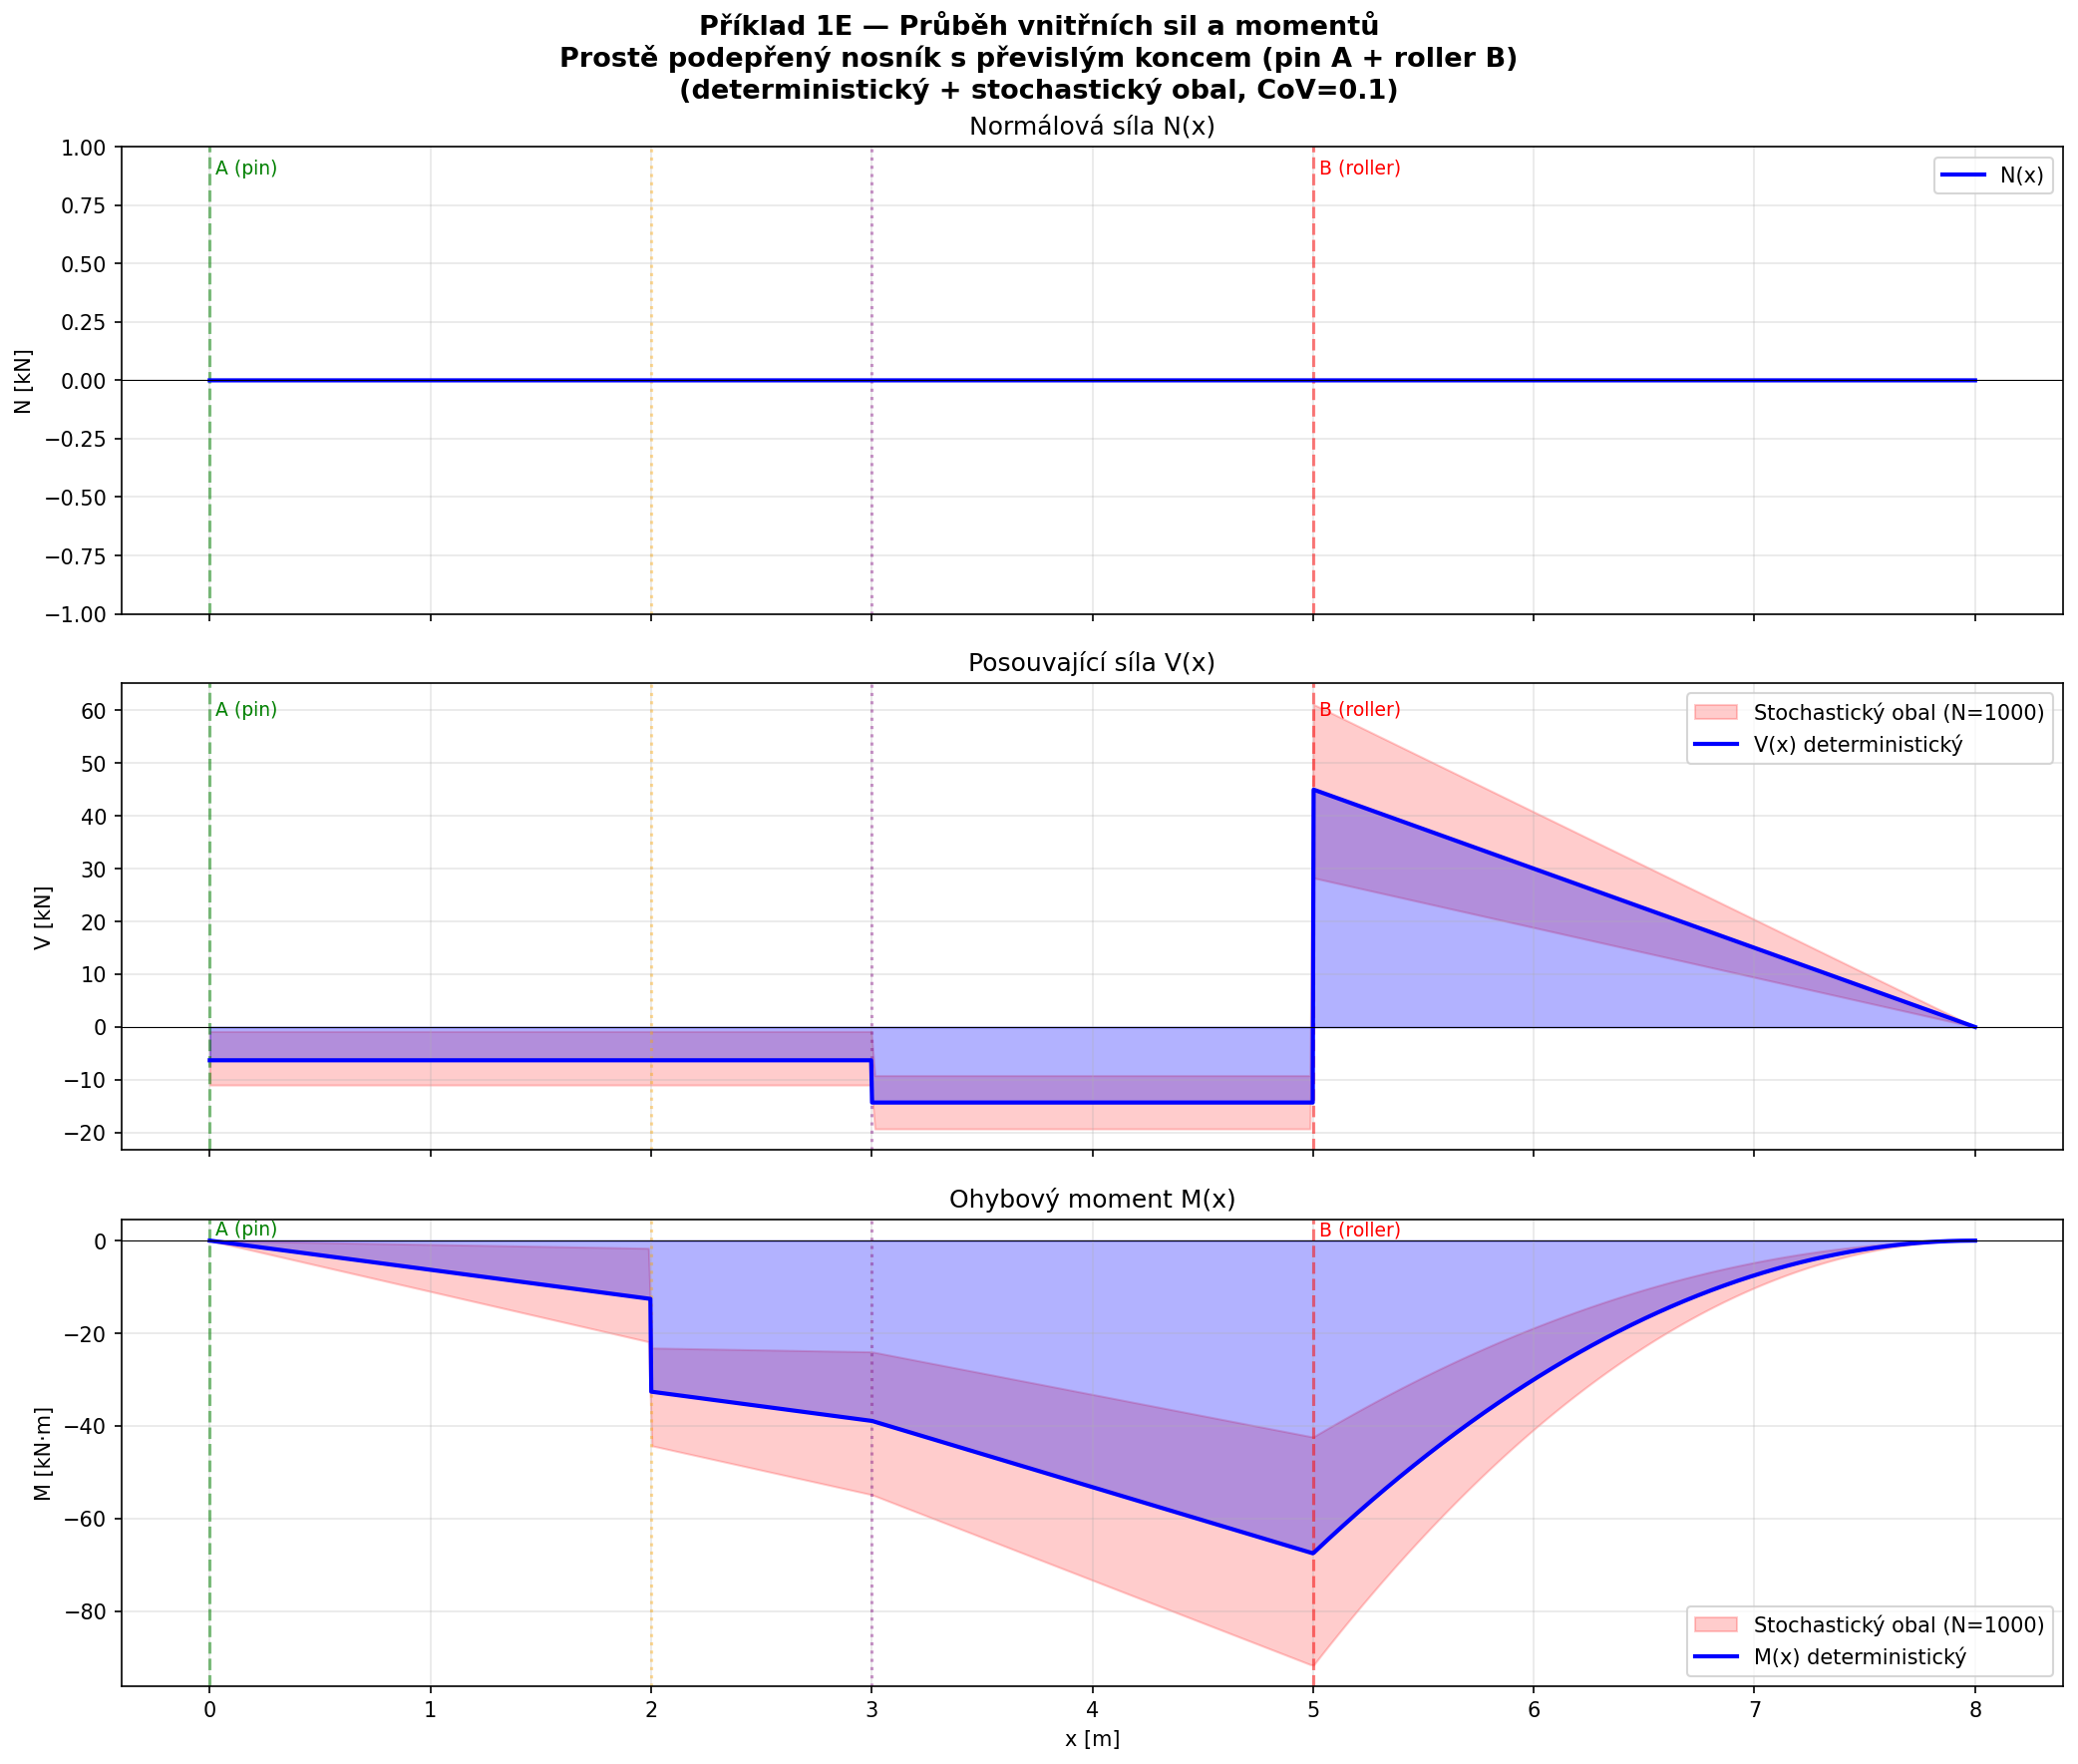
\includegraphics[width=\textwidth]{priklad_1E_diagram.png}
\caption{Průběh vnitřních sil $N(x)$, $V(x)$, $M(x)$ -- deterministická křivka (modrá) a~stochastický obal z~$1\,000$ realizací MC (červený pás)}
\label{fig:1E_diagram}
\end{figure}

\begin{figure}[H]
\centering
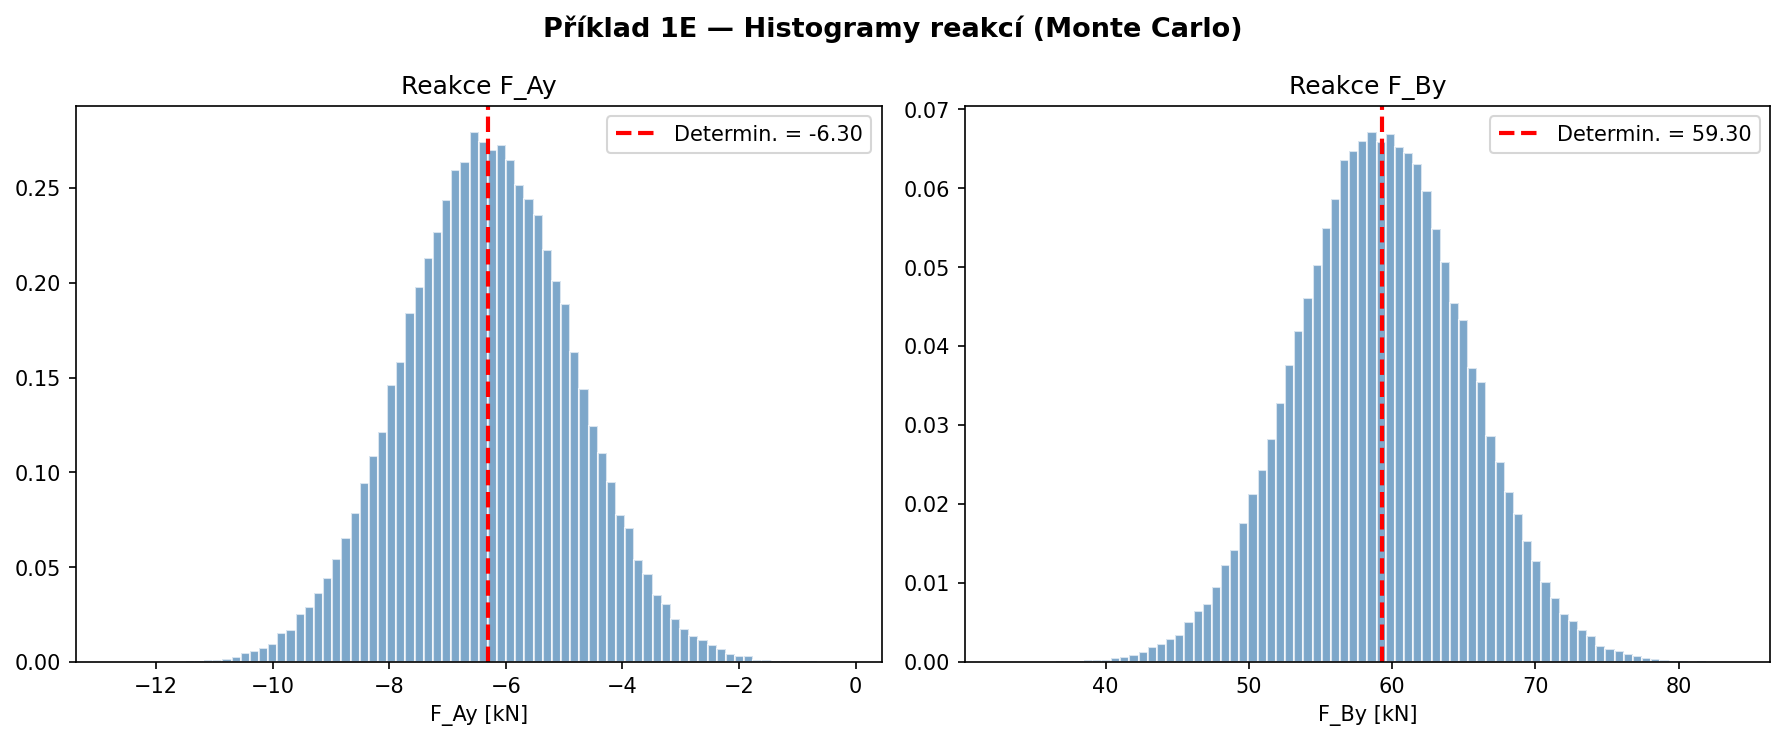
\includegraphics[width=\textwidth]{priklad_1E_histogramy.png}
\caption{Empirické histogramy reakcí $F_{Ay}$, $F_{By}$ z~Monte Carlo simulace ($N = 100\,000$). Červená přerušovaná čára značí deterministickou hodnotu, která odpovídá střední hodnotě histogramu}
\label{fig:1E_hist}
\end{figure}

\newpage
%% ============================================================
%% PŘÍKLAD 2E
%% ============================================================
\section{Příklad 2E -- Osový kvadratický moment nesymetrického průřezu}

\subsection{Zadání}

U~tělesa podle obrázku určete osový kvadratický moment k~ose $x$ a~$y$. Střední hodnoty rozměrů jsou uvedeny na obrázku, variační koeficient je $\mathrm{CoV} = 0{,}2$. Stochastické veličiny popisujte normálním rozdělením.

\subsection{Geometrie průřezu}

Jedná se o~\textbf{nesymetrický průřez} složený ze tří obdélníků (širší spodní pásnice, vlevo zarovnaná stojina, užší horní pásnice). Počátek souřadného systému je v~levém dolním rohu obalového obdélníku.

\medskip\noindent
Rozměry dílčích obdélníků:
\begin{itemize}[nosep]
    \item Spodní pásnice: $b_1 = 200\unit{mm}$, $h_1 = 30\unit{mm}$
    \item Stojina (zarovnaná k~levému okraji): $b_2 = 30\unit{mm}$, $h_2 = 140\unit{mm}$
    \item Horní pásnice: $b_3 = 100\unit{mm}$, $h_3 = 30\unit{mm}$
    \item 70\,mm = hloubka 3D tělesa (extruze), neovlivňuje 2D průřez
\end{itemize}

\begin{table}[H]
\centering
\caption{Rozměry a polohy dílčích obdélníků}
\begin{tabular}{lccccc}
\toprule
\textbf{Část} & $b_i$ [mm] & $h_i$ [mm] & $A_i$ [mm$^2$] & $x_{C,i}$ [mm] & $y_{C,i}$ [mm] \\
\midrule
Spodní pásnice (1) & 200 & 30 & 6\,000 & 100{,}0 & 15{,}0 \\
Stojina (2) & 30 & 140 & 4\,200 & 15{,}0 & 100{,}0 \\
Horní pásnice (3) & 100 & 30 & 3\,000 & 50{,}0 & 185{,}0 \\
\bottomrule
\end{tabular}
\end{table}

\subsection{Deterministické řešení}

\subsubsection{Plocha průřezu}

\begin{equation}
    A = A_1 + A_2 + A_3 = 6\,000 + 4\,200 + 3\,000 = \boxed{13\,200\unit{mm^2}}
\end{equation}

\subsubsection{Těžiště}

\begin{equation}
    x_C = \frac{\sum A_i \cdot x_{C,i}}{A} = \frac{6\,000 \cdot 100 + 4\,200 \cdot 15 + 3\,000 \cdot 50}{13\,200} = \frac{813\,000}{13\,200} = \boxed{61{,}59\unit{mm}}
\end{equation}

\begin{equation}
    y_C = \frac{\sum A_i \cdot y_{C,i}}{A} = \frac{6\,000 \cdot 15 + 4\,200 \cdot 100 + 3\,000 \cdot 185}{13\,200} = \frac{1\,065\,000}{13\,200} = \boxed{80{,}68\unit{mm}}
\end{equation}

\subsubsection{Těžišťové kvadratické momenty (Steinerova věta)}

\begin{equation}
    I_{x'} = \sum \left( \frac{b_i h_i^3}{12} + A_i \cdot (y_{C,i} - y_C)^2 \right)
\end{equation}

\begin{align}
    I_{x',1} &= \tfrac{200 \cdot 30^3}{12} + 6\,000 \cdot (15 - 80{,}68)^2 = 450\,000 + 25\,884\,595 = 26\,334\,595\unit{mm^4} \\
    I_{x',2} &= \tfrac{30 \cdot 140^3}{12} + 4\,200 \cdot (100 - 80{,}68)^2 = 6\,860\,000 + 1\,567\,408 = 8\,427\,408\unit{mm^4} \\
    I_{x',3} &= \tfrac{100 \cdot 30^3}{12} + 3\,000 \cdot (185 - 80{,}68)^2 = 225\,000 + 32\,646\,840 = 32\,871\,840\unit{mm^4}
\end{align}

\begin{equation}
    \boxed{I_{x'} = 26\,334\,595 + 8\,427\,408 + 32\,871\,840 = 67{,}63 \E{6}\unit{mm^4}}
\end{equation}

Analogicky pro $I_{y'}$:
\begin{align}
    I_{y',1} &= \tfrac{30 \cdot 200^3}{12} + 6\,000 \cdot (100 - 61{,}59)^2 = 20\,000\,000 + 8\,851\,553 = 28\,851\,553\unit{mm^4} \\
    I_{y',2} &= \tfrac{140 \cdot 30^3}{12} + 4\,200 \cdot (15 - 61{,}59)^2 = 315\,000 + 9\,116\,982 = 9\,431\,982\unit{mm^4} \\
    I_{y',3} &= \tfrac{30 \cdot 100^3}{12} + 3\,000 \cdot (50 - 61{,}59)^2 = 2\,500\,000 + 403\,047 = 2\,903\,047\unit{mm^4}
\end{align}

\begin{equation}
    \boxed{I_{y'} = 28\,851\,553 + 9\,431\,982 + 2\,903\,047 = 41{,}19 \E{6}\unit{mm^4}}
\end{equation}

\subsubsection{Kvadratické momenty k~vnějším osám (okraje obalového obdélníku)}

\begin{align}
    I_x &= I_{x'} + A \cdot y_C^2 = 67{,}63 \E{6} + 13\,200 \cdot 80{,}68^2 = \boxed{153{,}6 \E{6}\unit{mm^4}} \\
    I_y &= I_{y'} + A \cdot x_C^2 = 41{,}19 \E{6} + 13\,200 \cdot 61{,}59^2 = \boxed{91{,}3 \E{6}\unit{mm^4}}
\end{align}

\subsection{Stochastická analýza}

Rozměrové veličiny ($b_i$, $h_i$) mají normální rozdělení s~$\mathrm{CoV} = 0{,}2$. Monte Carlo simulace ($N = 100\,000$):

\begin{table}[H]
\centering
\caption{Statistiky těžišťových kvadratických momentů (MC, $N = 10^5$)}
\begin{tabular}{lcccc}
\toprule
\textbf{Veličina} & $\boldsymbol{\mu}$ [$\E{6}$ mm$^4$] & $\boldsymbol{\sigma}$ [$\E{6}$ mm$^4$] & \textbf{CoV} & \textbf{95\% CI} [$\E{6}$ mm$^4$] \\
\midrule
$I_{x'}$ & 69{,}19 & 28{,}80 & 0{,}416 & $[24{,}9;\; 135{,}9]$ \\
$I_{y'}$ & 45{,}62 & 25{,}47 & 0{,}558 & --- \\
\bottomrule
\end{tabular}
\end{table}

\noindent\textbf{Poznámka:} CoV výstupu ($0{,}42$--$0{,}56$) výrazně převyšuje vstupní CoV ($0{,}2$), protože $I$ závisí na rozměrech ve třetí mocnině (zesílení nejistoty). Vyšší CoV pro $I_{y'}$ odráží silnější citlivost na šířky pásnic ($b^3$).

\begin{figure}[H]
\centering
\begin{subfigure}[b]{0.48\textwidth}
    
\includegraphics[width=\textwidth]{priklad_2E_profil.png}
    \caption{Geometrie L-profilu s~těžištěm}
\end{subfigure}
\hfill
\begin{subfigure}[b]{0.48\textwidth}
    
\includegraphics[width=\textwidth]{priklad_2E_histogramy.png}
    \caption{Histogramy $I_x$ a $I_y$}
\end{subfigure}
\caption{Příklad 2E -- L-profil (rovnoramenný úhelník)}
\end{figure}

\newpage
%% ============================================================
%% PŘÍKLAD 3E
%% ============================================================
\section{Příklad 3E -- Pravděpodobnost bezporuchového provozu klínových řemenů}

\subsection{Zadání}

V~klínových řemenech byla zjištěna provozní napětí $S$ [MPa] a~meze pevnosti $R$ [MPa]:

\medskip
\noindent\textbf{Provozní napětí $S$} ($n = 10$): 223; 116; 158{,}5; 199; 136{,}5; 169{,}5; 267{,}5; 127; 184; 151

\noindent\textbf{Mez pevnosti $R$} ($n = 12$): 211; 269{,}5; 192; 301{,}5; 220{,}5; 243{,}5; 182{,}5; 257; 234; 199{,}5; 216; 205

\medskip
\noindent Jaká je pravděpodobnost bezporuchového provozu?

\subsection{Statistický popis dat}

\begin{table}[H]
\centering
\caption{Základní statistiky naměřených dat}
\begin{tabular}{lcccc}
\toprule
\textbf{Veličina} & $\boldsymbol{\bar{x}}$ [MPa] & $\boldsymbol{s}$ [MPa] & \textbf{CoV} & \textbf{Shapiro-Wilk $p$} \\
\midrule
Provozní napětí $S$ & 173{,}20 & 46{,}70 & 0{,}270 & 0{,}640 (normální $\checkmark$) \\
Mez pevnosti $R$ & 227{,}67 & 34{,}95 & 0{,}154 & 0{,}589 (normální $\checkmark$) \\
\bottomrule
\end{tabular}
\end{table}

Shapiro-Wilkův test na hladině $\alpha = 0{,}05$ potvrzuje normalitu obou souborů.

\subsection{Analytický výpočet}

Bezporuchový provoz nastává, když mez pevnosti překoná provozní napětí: $R > S$. Definujeme \textbf{rezervu spolehlivosti}:
\begin{equation}
    Z = R - S
\end{equation}

Jsou-li $R \sim N(\mu_R, \sigma_R)$ a $S \sim N(\mu_S, \sigma_S)$ nezávislé, pak:
\begin{equation}
    Z \sim N\!\left(\mu_R - \mu_S,\; \sqrt{\sigma_R^2 + \sigma_S^2}\right)
\end{equation}

\begin{align}
    \mu_Z &= 227{,}67 - 173{,}20 = 54{,}47\unit{MPa} \\
    \sigma_Z &= \sqrt{34{,}95^2 + 46{,}70^2} = 58{,}33\unit{MPa}
\end{align}

\textbf{Index spolehlivosti:}
\begin{equation}
    \beta = \frac{\mu_Z}{\sigma_Z} = \frac{54{,}47}{58{,}33} = \boxed{0{,}934}
\end{equation}

\textbf{Pravděpodobnost poruchy:}
\begin{equation}
    P_f = \Phi(-\beta) = \Phi(-0{,}934) = 0{,}1752 = 17{,}52\%
\end{equation}

\textbf{Pravděpodobnost bezporuchového provozu:}
\begin{equation}
    \boxed{P_s = 1 - P_f = 0{,}8248 = 82{,}48\%}
\end{equation}

\subsection{Monte Carlo simulace}

Simulace s~$N = 1\,000\,000$ realizací potvrzuje analytický výsledek:

\begin{table}[H]
\centering
\caption{Srovnání metod výpočtu}
\begin{tabular}{lc}
\toprule
\textbf{Metoda} & $\boldsymbol{P_s}$ [\%] \\
\midrule
Analyticky (normální) & 82{,}48 \\
Monte Carlo (normální) & 82{,}45 \\
Monte Carlo (log-normální) & 83{,}39 \\
\bottomrule
\end{tabular}
\end{table}

\begin{figure}[H]
\centering
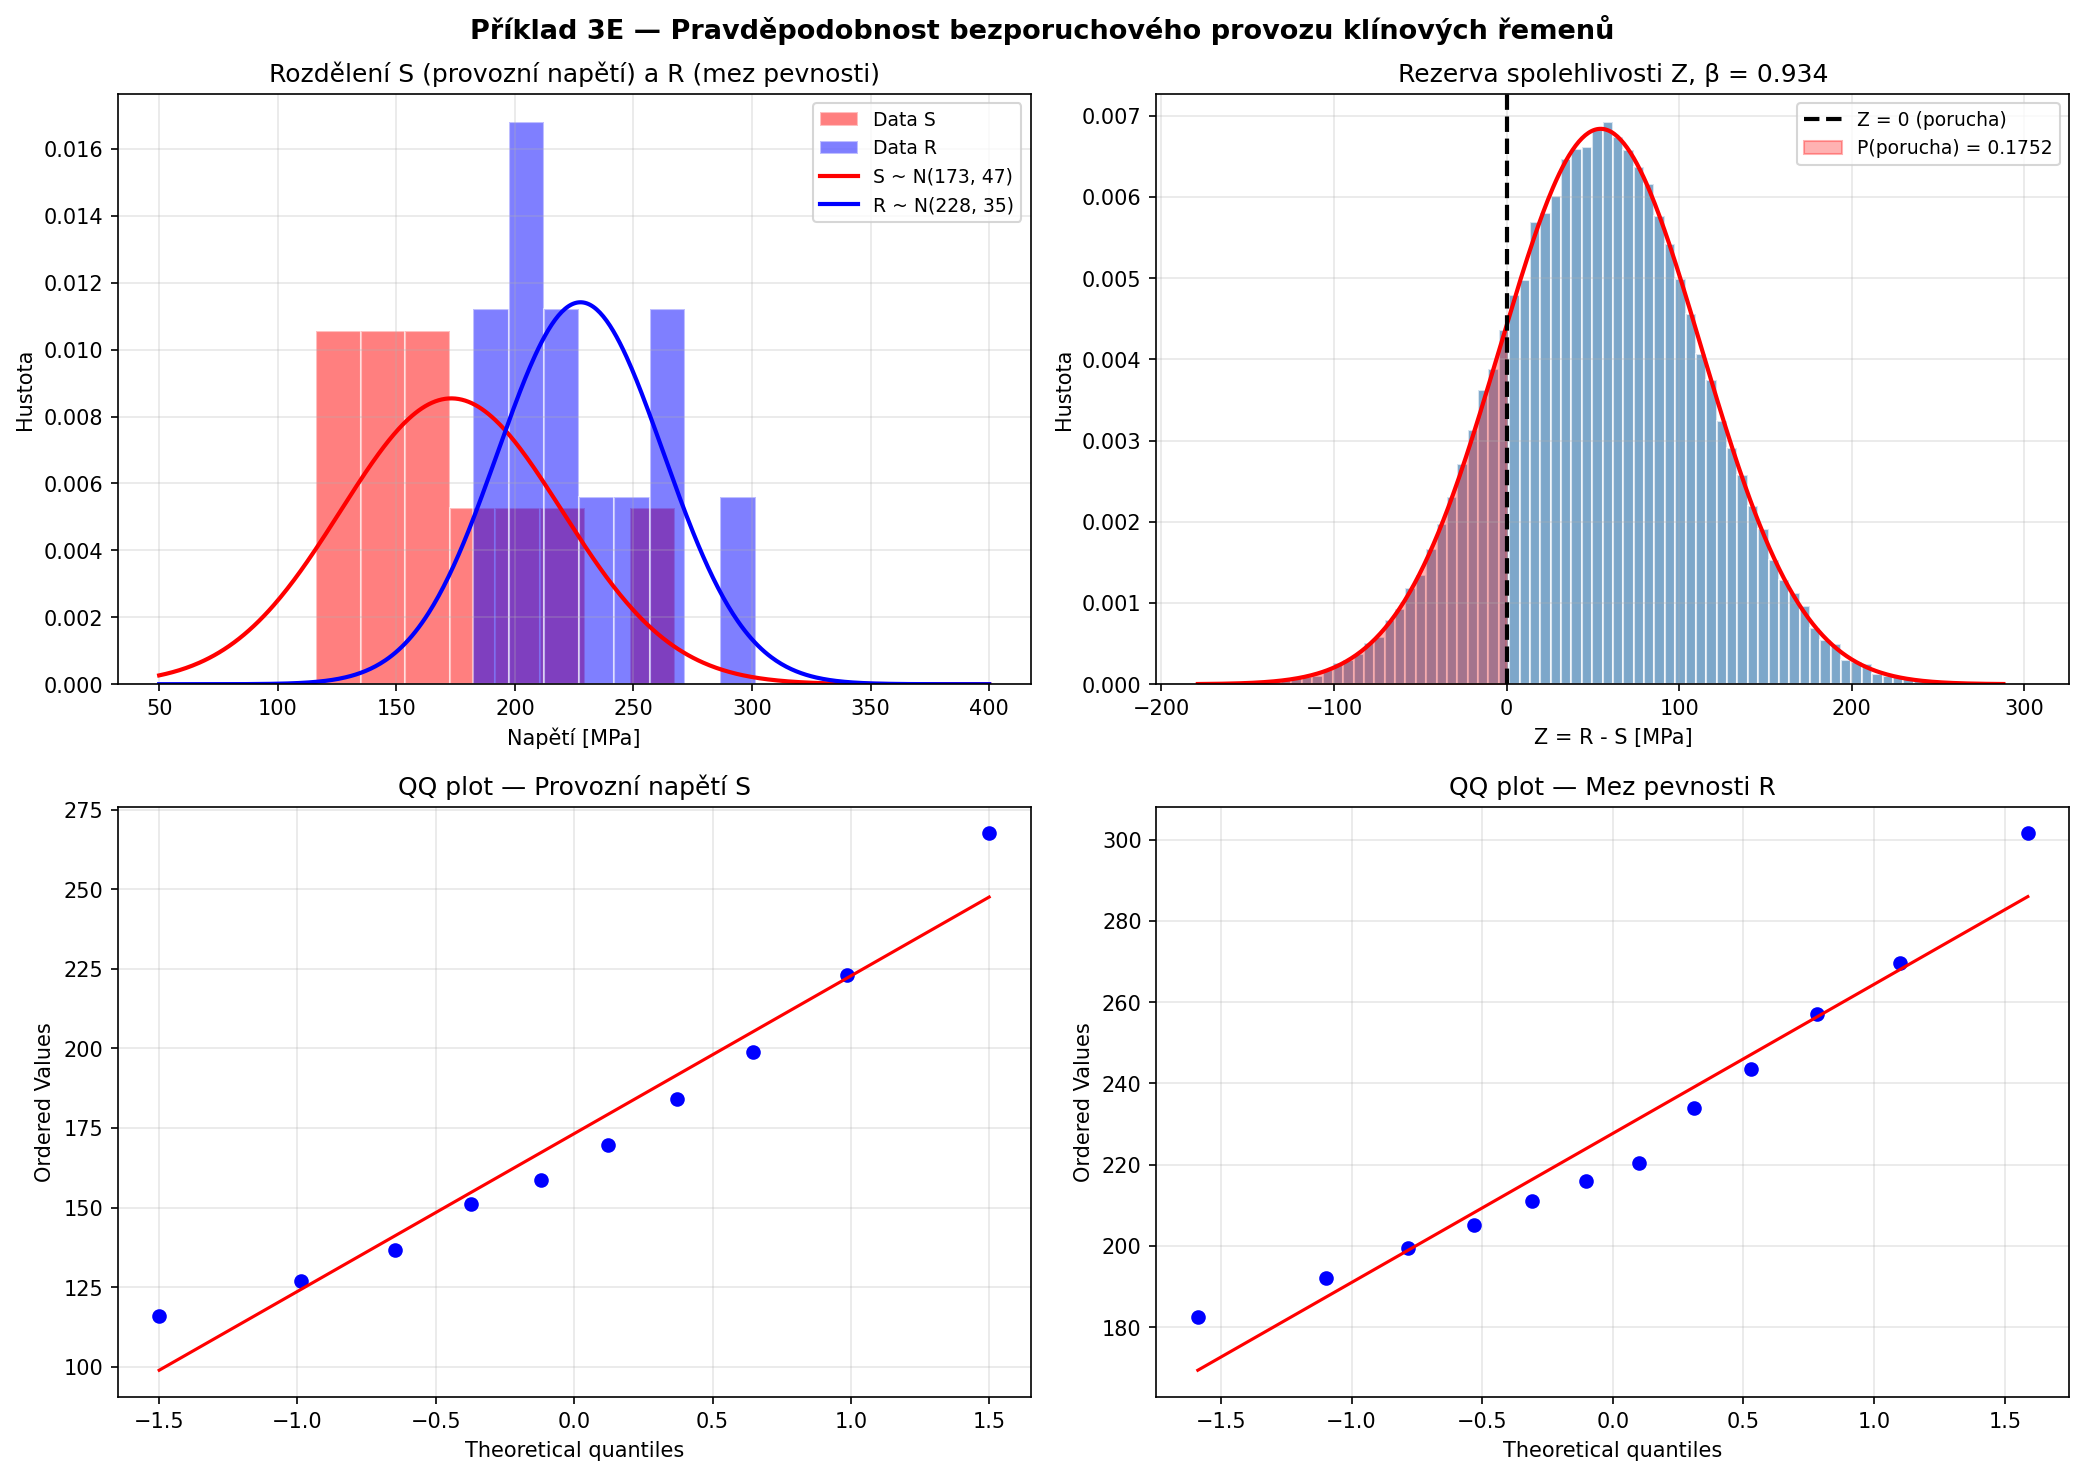
\includegraphics[width=\textwidth]{priklad_3E_vysledky.png}
\caption{Příklad 3E -- Rozdělení $S$, $R$, rezerva $Z$, QQ ploty}
\label{fig:3E}
\end{figure}

\newpage
%% ============================================================
%% PŘÍKLAD 4E
%% ============================================================
\section{Příklad 4E -- MS pružnosti a deformace stupňovitého prutu}

\subsection{Zadání}

Určete pravděpodobnost dosažení mezního stavu pružnosti a~mezního stavu deformace. Proveďte citlivostní analýzu.

\begin{itemize}[nosep]
    \item $R_e = 500\unit{MPa}$, $w_{\max} = 2\unit{mm}$, $M = 100\unit{N \cdot m}$
    \item Tloušťka $t = 15\unit{mm}$
    \item Stupňovitý plochý prut, výšky úseků $h_1 = 45\unit{mm}$, $h_2 = 30\unit{mm}$, $h_3 = 10\unit{mm}$
    \item Poloměry přechodů: $r_1 = 3\unit{mm}$ (45$\to$30), $r_2 = 6\unit{mm}$ (30$\to$10)
    \item Délky úseků (odhad z výkresu): $L_1 = 60$, $L_2 = 80$, $L_3 = 60\unit{mm}$
    \item Stochastické veličiny: log-normální rozdělení, $\mathrm{CoV} = 0{,}1$
\end{itemize}

\subsection{Deterministické řešení}

\subsubsection{Nominální napětí v~jednotlivých úsecích}

Průřezové moduly $W_i = t \cdot h_i^2 / 6$ a~nominální napětí $\sigma_{\mathrm{nom},i} = M/W_i$:

\begin{table}[H]
\centering
\begin{tabular}{cccc}
\toprule
\textbf{Úsek} & $h_i$ [mm] & $W_i$ [mm$^3$] & $\sigma_{\mathrm{nom},i}$ [MPa] \\
\midrule
1 & 45 & 5\,062{,}5 & 19{,}75 \\
2 & 30 & 2\,250{,}0 & 44{,}44 \\
3 & 10 & 250{,}0 & \textbf{400{,}00} \\
\bottomrule
\end{tabular}
\end{table}

Kritická sekce je úsek 3 ($h_3 = 10\unit{mm}$).

\subsubsection{Součinitelé tvaru (Peterson, stupňovitý plochý prut v~ohybu)}

\begin{itemize}[nosep]
    \item Vrub $r_1$ (45$\to$30): $D/d = 1{,}5$, $r/d = 0{,}1 \Rightarrow K_{t1} \approx 1{,}68$
    \item Vrub $r_2$ (30$\to$10): $D/d = 3{,}0$, $r/d = 0{,}6 \Rightarrow K_{t2} \approx 1{,}15$
\end{itemize}

\subsubsection{Maximální napětí}

\begin{align}
    \sigma_{\max,1} &= K_{t1} \cdot \sigma_{\mathrm{nom},2} = 1{,}68 \cdot 44{,}44 = 74{,}7\unit{MPa} \\
    \sigma_{\max,2} &= K_{t2} \cdot \sigma_{\mathrm{nom},3} = 1{,}15 \cdot 400 = \boxed{460\unit{MPa}}
\end{align}

Rozhoduje vrub $r_2$. Součinitel bezpečnosti k~MS pružnosti:
\begin{equation}
    k = \frac{R_e}{\sigma_{\max,2}} = \frac{500}{460} = \boxed{1{,}087}
\end{equation}

\subsubsection{Průhyb (Mohrova analogie pro stupňovitý prut)}

Kvadratické momenty $I_i = t \cdot h_i^3 / 12$:
\begin{equation}
    I_1 = 113\,906, \quad I_2 = 33\,750, \quad I_3 = 1\,250\unit{mm^4}
\end{equation}

Konzola s~konstantním momentem $M$ (vetknutí u $h_1$, volný konec za $h_3$):
\begin{equation}
    w = \frac{M}{E} \sum_{i=1}^{3} \frac{1}{I_i} \cdot \frac{(L - a_i)^2 - (L - b_i)^2}{2}
\end{equation}
kde $L = L_1 + L_2 + L_3 = 200\unit{mm}$, $[a_i, b_i]$ jsou meze úseku $i$. Po dosazení (sekce~3 dominuje, $\approx 81\,\%$ příspěvku):
\begin{equation}
    w = 0{,}043 + 0{,}113 + 0{,}686 = \boxed{0{,}842\unit{mm}} < w_{\max} = 2\unit{mm}
\end{equation}

\subsection{Stochastická analýza (Monte Carlo)}

Všechny vstupy: log-normální, $\mathrm{CoV} = 0{,}1$, simulace $N = 500\,000$.

\subsubsection{MS pružnosti: $g_1 = R_e - \sigma_{\max} > 0$}

\begin{align}
    P(\text{porucha MS pružnosti}) &= P(\sigma_{\max} > R_e) = \boxed{39{,}6\,\%} \\
    \beta_{\mathrm{yield}} &\approx 0{,}26
\end{align}

Deterministicky $\sigma_{\max} = 460$ MPa leží těsně pod $R_e = 500$ MPa, ale velký rozptyl ($\sigma_{\sigma_{\max}} \approx 128$ MPa) vede k~vysoké pravděpodobnosti poruchy. \textbf{Součást nevyhovuje.}

\subsubsection{MS deformace: $g_2 = w_{\max} - w > 0$}

\begin{align}
    P(\text{porucha MS deformace}) &\approx \boxed{0{,}47\,\%} \\
    \beta_{\mathrm{deform}} &\approx 2{,}60
\end{align}

MS deformace s~rezervou vyhovuje.

\subsection{Citlivostní analýza}

\begin{table}[H]
\centering
\caption{Faktory důležitosti (importance factors) pro MS pružnosti}
\begin{tabular}{lcc}
\toprule
\textbf{Veličina} & $\boldsymbol{\rho}(g_1, X_i)$ & $\boldsymbol{\alpha_i^2}$ [\%] \\
\midrule
$h_3$ & $+0{,}683$ & \textbf{48{,}8} \\
$R_e$ & $+0{,}365$ & 13{,}9 \\
$M$ & $-0{,}345$ & 12{,}5 \\
$K_{t2}$ & $-0{,}345$ & 12{,}4 \\
$t$ & $+0{,}343$ & 12{,}3 \\
\bottomrule
\end{tabular}
\end{table}

\noindent\textbf{Závěr citlivostní analýzy:} Dominantní vliv má výška kritického průřezu $h_3$ (49\,\%) díky kvadratické závislosti $\sigma \propto 1/h^2$. Ostatní veličiny mají rovnoměrný příspěvek $\sim 12\,\%$. Pro zvýšení spolehlivosti je nejúčinnější zvětšit $h_3$ nebo snížit jeho toleranci.

\begin{figure}[H]
\centering

\includegraphics[width=\textwidth]{priklad_4E_vysledky.png}
\caption{Příklad 4E -- MS pružnosti a deformace, citlivostní analýza}
\label{fig:4E}
\end{figure}

\newpage
%% ============================================================
%% PŘÍKLAD 5E
%% ============================================================
\section{Příklad 5E -- Časový průběh napětí ve vrubech}

\subsection{Zadání}

Rotační hřídel se dvěma zápichy, axiálně zatížená střídavou silou s~obdélníkovým časovým průběhem.

\textbf{Geometrie} (z~výkresu, celková délka $L_{\mathrm{tot}} = 820\unit{mm}$):
\begin{itemize}[nosep]
    \item Hlavní průměr $D = 50\unit{mm}$, průměr v~zápichu $d = 35\unit{mm}$
    \item Poloměr zápichu $r = 5\unit{mm}$, šířka zápichu $10\unit{mm}$
    \item Úseky: $200 + 10 + 400 + 10 + 200\unit{mm}$
    \item Síla působí v~$x_F = 500\unit{mm}$ od levého vetknutí
    \item Levý vrub: $x \in [200; 210]\unit{mm}$ (před silou)
    \item Pravý vrub: $x \in [610; 620]\unit{mm}$ (za silou)
\end{itemize}

\textbf{Uložení:}
\begin{itemize}[nosep]
    \item \textbf{Vlevo:} pevné vetknutí (přenese tah i tlak).
    \item \textbf{Vpravo:} jednostranný kontakt s~tuhou stěnou ($\delta = 0$). Posuv do stěny nemožný, od stěny volný — pravá podpora přenáší pouze tlak.
\end{itemize}

\textbf{Zatížení:} obdélníková střídavá osová síla $F = \pm 1{,}4\cdot 10^5\unit{N}$, tolerance velikosti síly $+1000/-0\unit{N}$. Tolerance geometrie $\pm 0{,}5\unit{mm}$ na všech rozměrech.

\textbf{Cíl:} stanovit časový průběh lokálního napětí v~obou vrubech (statický výpočet, $K_t$).

\subsection{Deterministické řešení}

\subsubsection{Mechanika jednostranného kontaktu — dva zatěžovací stavy}

Jednostranný kontakt rozštěpí každou půlvlnu na odlišný staticky/staticky-neurčitý úkol:

\begin{center}
\begin{tabular}{lll}
\toprule
\textbf{Stav} & \textbf{Smysl síly} & \textbf{Pravý kontakt} \\
\midrule
A & $F = +140\unit{kN}$ (do stěny) & aktivní (tlakový), úloha staticky neurčitá \\
B & $F = -140\unit{kN}$ (od stěny) & odlepen, úloha staticky určitá \\
\bottomrule
\end{tabular}
\end{center}

\subsubsection{Stav A — staticky neurčitá úloha (kontakt aktivní)}

Konvence: tah pozitivní, $+x$ doprava. Označme $R_R$ reakci od pravé stěny (působí v~$-x$, tedy $R_R \le 0$).

Z~FBD pravé části hřídele plyne vnitřní osová síla:
\begin{align}
    N_{\mathrm{levá}}(x < x_F) &= F + R_R \\
    N_{\mathrm{pravá}}(x > x_F) &= R_R
\end{align}

\textbf{Podmínka kompatibility} (pravý konec se nepohne, $\Delta_{\mathrm{tot}} = 0$):
\begin{equation}
    N_{\mathrm{levá}} \cdot C_L + N_{\mathrm{pravá}} \cdot C_R = 0
\end{equation}
kde $C_L$, $C_R$ jsou osové poddajnosti levé a~pravé části (násobeno $E$):
\begin{align}
    A_D &= \frac{\pi D^2}{4} = 1963{,}5\unit{mm^2}, \quad A_d = \frac{\pi d^2}{4} = 962{,}1\unit{mm^2} \\
    C_L &= \frac{490}{A_D} + \frac{10}{A_d} = 0{,}24955 + 0{,}01039 = 0{,}25995\unit{mm/mm^2} \\
    C_R &= \frac{310}{A_D} + \frac{10}{A_d} = 0{,}15788 + 0{,}01039 = 0{,}16827\unit{mm/mm^2}
\end{align}

(Levá část: $200\unit{mm}$ v~$D$ + $10\unit{mm}$ v~$d$ + $290\unit{mm}$ v~$D$ = $490\unit{mm}$ v~$D$ + $10\unit{mm}$ v~$d$. Pravá část: $110 + 10 + 200$ v~$D/d$.)

Řešení:
\begin{align}
    R_R &= -F \cdot \frac{C_L}{C_L + C_R} = -140000 \cdot \frac{0{,}25995}{0{,}42822} = -84\,985\unit{N} \\
    N_{\mathrm{levá}}^A &= F + R_R = +55\,015\unit{N} \quad (\text{tah}) \\
    N_{\mathrm{pravá}}^A &= R_R = -84\,985\unit{N} \quad (\text{tlak})
\end{align}

\subsubsection{Stav B — staticky určitá úloha (kontakt rozevřen)}

Pravý konec se odlepí, $R_R = 0$. Z~rovnováhy:
\begin{align}
    N_{\mathrm{levá}}^B &= F + 0 = -140\,000\unit{N} \quad (\text{tlak}) \\
    N_{\mathrm{pravá}}^B &= 0
\end{align}

\subsubsection{Součinitel koncentrace napětí}

Geometrické poměry pro Petersonův graf (Chart 2.19, kruhový hřídel s~U-vrubem, axiální tah):
\begin{equation}
    \frac{D}{d} = 1{,}429, \qquad \frac{r}{d} = 0{,}143 \quad\Rightarrow\quad \boxed{K_t \approx 2{,}10}
\end{equation}

(Neuberova aproximace $K_t = 1 + 2\sqrt{t/r} = 3{,}449$ je horní konzervativní mez; Petersonův graf preferován jako přesnější.)

\subsubsection{Lokální napětí ve vrubech}

\textbf{Levý vrub} (v~levé části, působí oba stavy):
\begin{align}
    \sigma_{\mathrm{L}}^A &= K_t \cdot \frac{N_{\mathrm{levá}}^A}{A_d} = 2{,}10 \cdot \frac{55\,015}{962{,}1} = \boxed{+120{,}1\unit{MPa}} \\
    \sigma_{\mathrm{L}}^B &= K_t \cdot \frac{N_{\mathrm{levá}}^B}{A_d} = 2{,}10 \cdot \frac{-140\,000}{962{,}1} = \boxed{-305{,}6\unit{MPa}}
\end{align}

\textbf{Pravý vrub} (v~pravé části, působí jen Stav~A):
\begin{align}
    \sigma_{\mathrm{R}}^A &= K_t \cdot \frac{N_{\mathrm{pravá}}^A}{A_d} = 2{,}10 \cdot \frac{-84\,985}{962{,}1} = \boxed{-185{,}5\unit{MPa}} \\
    \sigma_{\mathrm{R}}^B &= 0\unit{MPa}
\end{align}

\subsection{Časový průběh napětí}

Síla $F(t)$ obdélníkově střídá hodnoty $+140\unit{kN}$ a~$-140\unit{kN}$. Statický výpočet $\Rightarrow$ napětí mezi dvěma diskrétními hodnotami:

\begin{center}
\begin{tabular}{lcccccc}
\toprule
\textbf{Vrub} & $\sigma_{\max}$ & $\sigma_{\min}$ & $\sigma_a$ & $\sigma_m$ & $R = \sigma_{\min}/\sigma_{\max}$ & \textbf{Charakter cyklu} \\
\midrule
Levý  & $+120{,}1$ & $-305{,}6$ & $212{,}8$ & $-92{,}8$ & $-2{,}55$ & asymetrický střídavý \\
Pravý & $0$        & $-185{,}5$ & $92{,}8$  & $-92{,}8$ & $\pm\infty$ & míjivý tlak (0 $\leftrightarrow$ tlak) \\
\bottomrule
\end{tabular}
\end{center}

\textbf{Pozorování:}
\begin{itemize}[nosep]
    \item Levý vrub má dominantní tlakovou špičku $-305{,}6\unit{MPa}$ ze Stavu~B (kontakt odlepen, celá síla působí proti levému vetknutí).
    \item Pravý vrub je vždy v~tlaku nebo bez napětí. Při Stavu~B je $\sigma = 0$ exaktně, protože pravá část je za místem působení síly a~kontakt je neaktivní.
    \item Obě střední napětí $\sigma_m$ jsou shodně $-92{,}8\unit{MPa}$ (důsledek vyvážených sil).
\end{itemize}

\subsection{Stochastická analýza}

Rozměry s~tolerancí $\pm 0{,}5\unit{mm}$: $\sigma_{\mathrm{dim}} = 0{,}5/3 \approx 0{,}167\unit{mm}$ (pravidlo $3\sigma$, normální rozdělení). Síla $F \sim \mathcal{U}(140\,000;\,141\,000)\unit{N}$ (uniformní, dle tolerance $+1000/-0$). Náhodné: $D, d, r$, všech 5 délek úseků, poloha síly $x_F$, velikost síly $F$.

\begin{table}[H]
\centering
\caption{Statistiky napětí v~obou vrubech ($N = 100\,000$)}
\begin{tabular}{lccccc}
\toprule
\textbf{Veličina} & $\boldsymbol{\mu}$ & $\boldsymbol{\sigma}$ & \textbf{CoV} & \textbf{95\% CI} \\
\midrule
$\sigma_{\mathrm{L,max}}$ [MPa] & $+120{,}54$ & $1{,}91$ & $0{,}016$ & $[+116{,}85;\; +124{,}33]$ \\
$\sigma_{\mathrm{L,min}}$ [MPa] & $-306{,}74$ & $4{,}80$ & $0{,}016$ & $[-316{,}32;\; -297{,}44]$ \\
$\sigma_{\mathrm{L},a}$    [MPa] & $+213{,}64$ & $3{,}35$ & $0{,}016$ & $[+207{,}15;\; +220{,}32]$ \\
$\sigma_{\mathrm{R,min}}$ [MPa] & $-186{,}20$ & $2{,}91$ & $0{,}016$ & $[-192{,}00;\; -180{,}59]$ \\
$\sigma_{\mathrm{R},a}$    [MPa] & $+93{,}10$  & $1{,}45$ & $0{,}016$ & $[+90{,}29;\; +96{,}00]$ \\
$K_t$ [-] & $2{,}100$ & $0{,}020$ & $0{,}010$ & $[2{,}06;\; 2{,}14]$ \\
\bottomrule
\end{tabular}
\end{table}

Variabilita napětí $\mathrm{CoV} \approx 1{,}6\%$ — nízká, dominuje rozptyl $A_d$ (kvadratická závislost na $d$) a~$K_t$ (citlivost na $r$). Rozptyl síly přispívá řádově $0{,}2\%$ (úzká tolerance).

\begin{figure}[H]
\centering
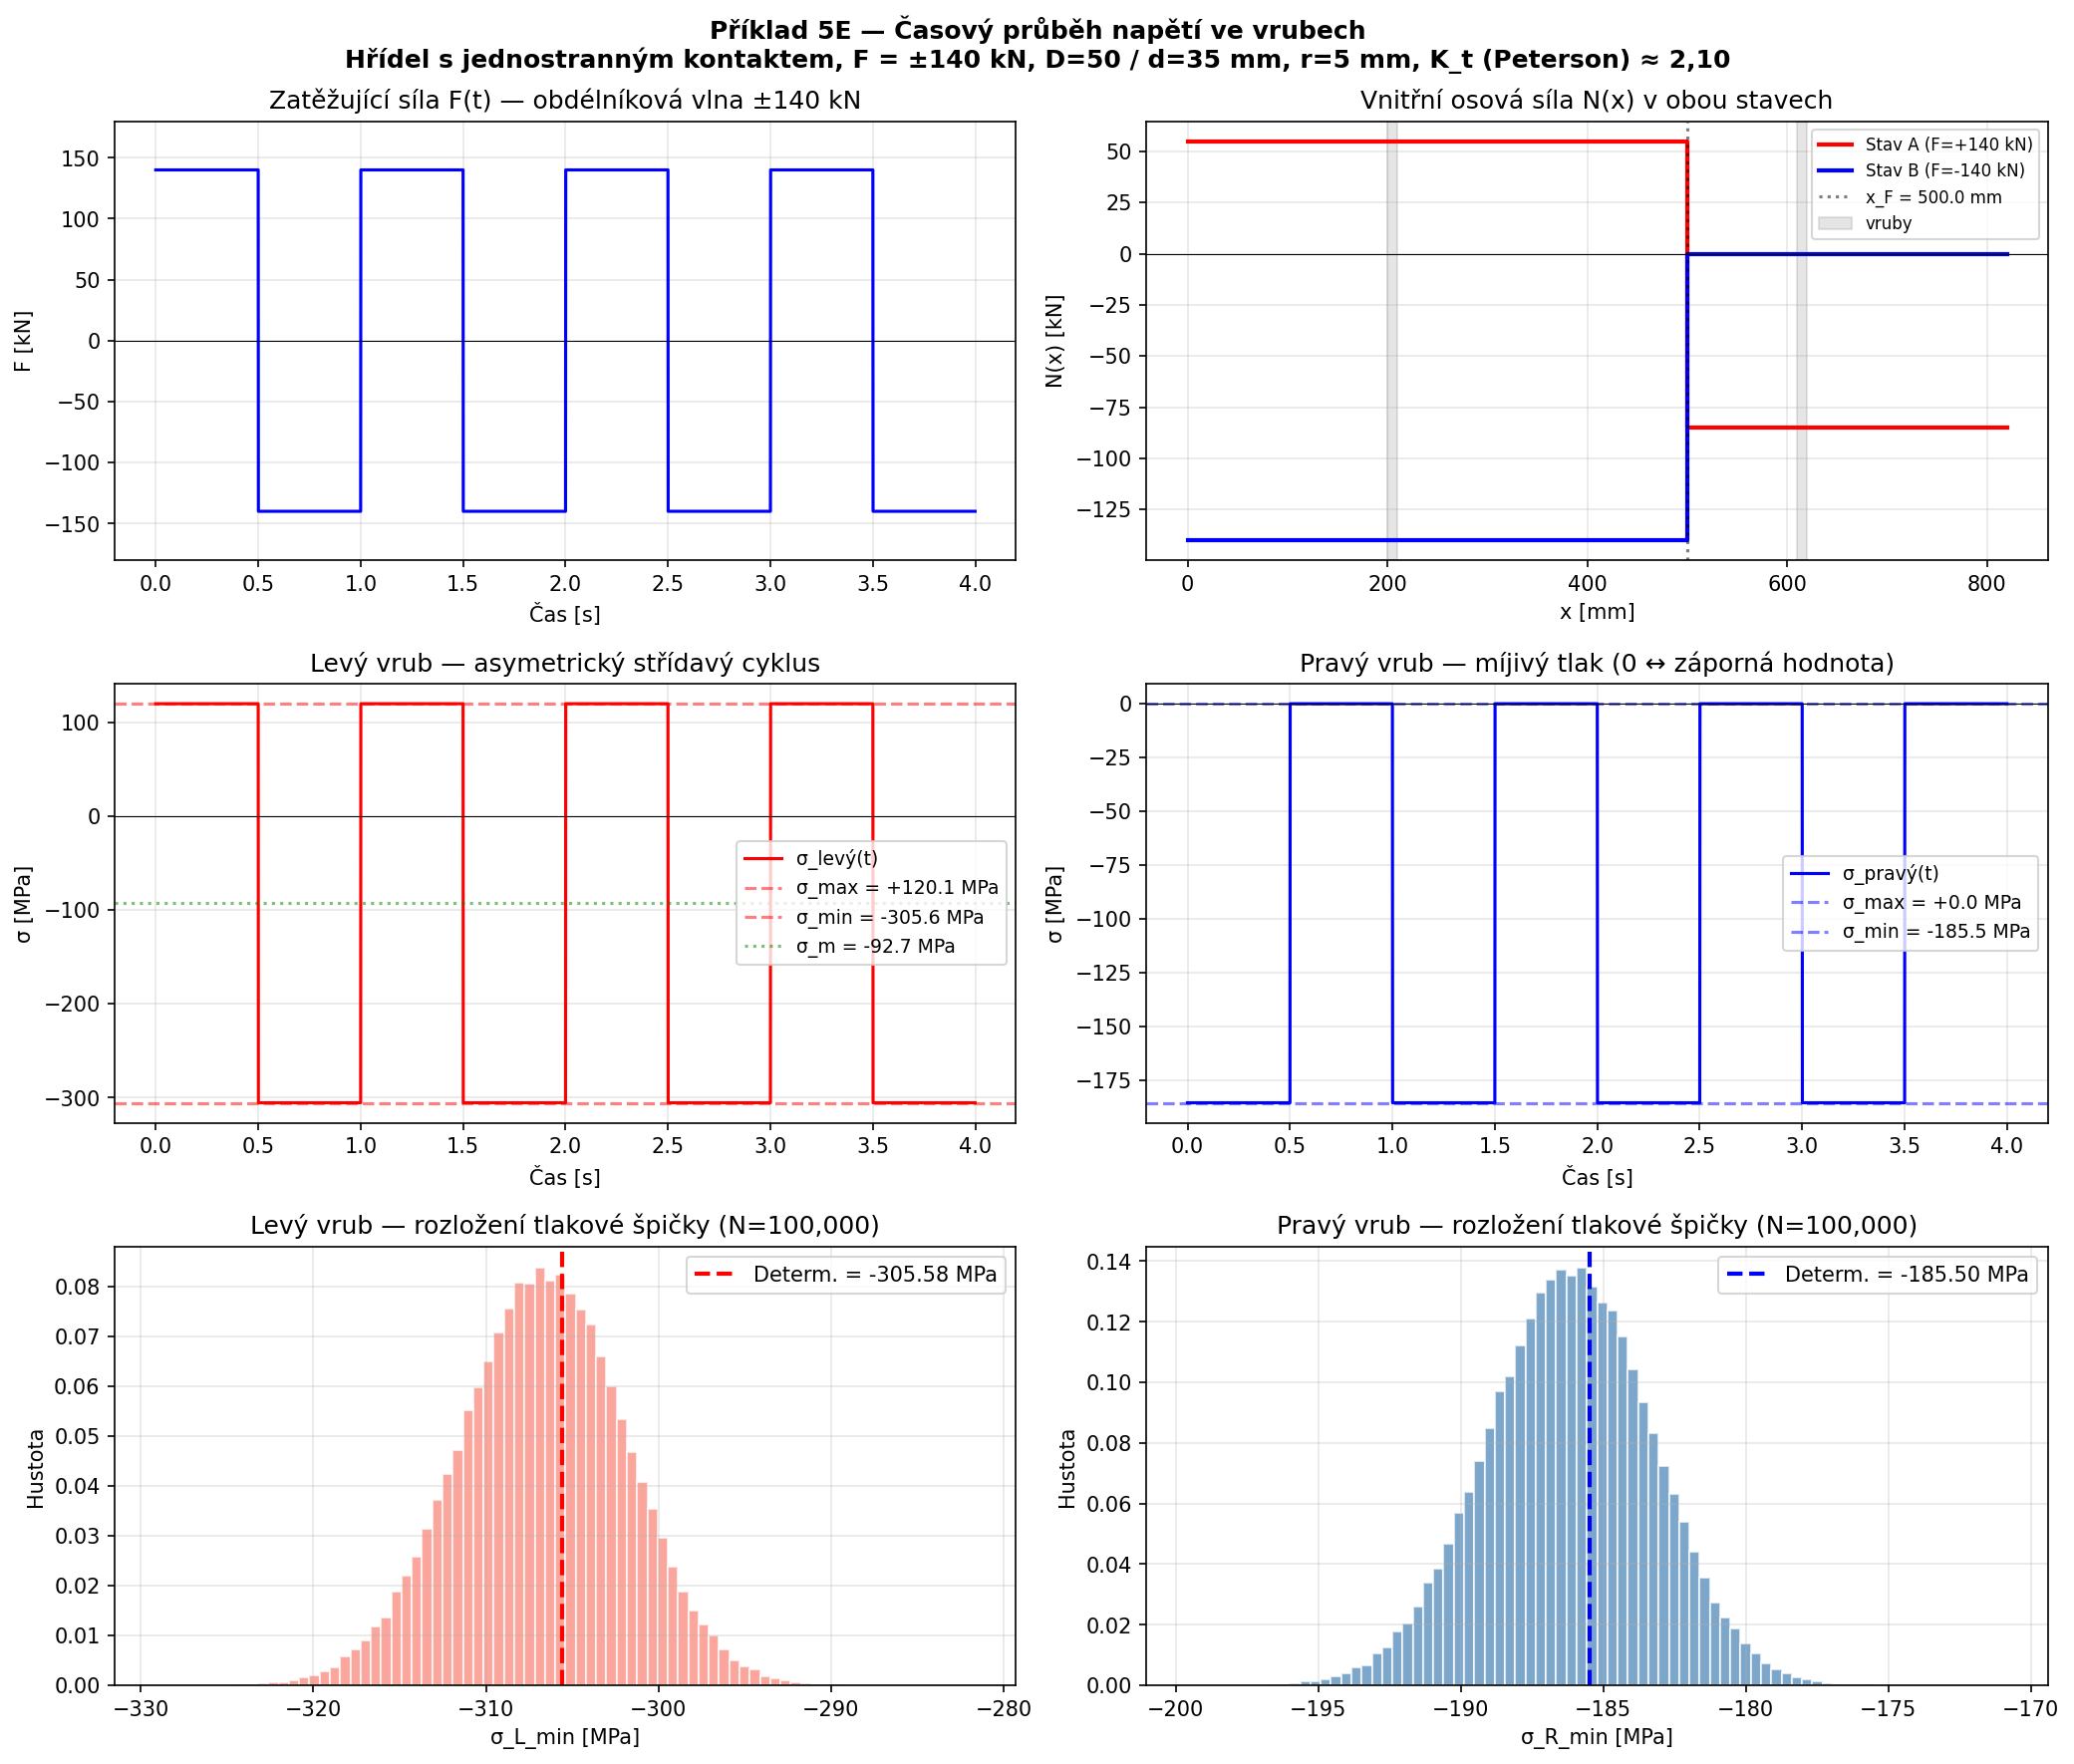
\includegraphics[width=\textwidth]{priklad_5E_vysledky.png}
\caption{Příklad 5E -- Časový průběh síly a~napětí, stochastická analýza}
\label{fig:5E}
\end{figure}

\begin{figure}[H]
\centering

\includegraphics[width=0.65\textwidth]{priklad_5E_haigh.png}
\caption{Příklad 5E -- Haighův diagram ($\sigma_a$ vs $\sigma_m$) s~Goodmanovou přímkou}
\label{fig:5E_haigh}
\end{figure}

\newpage
%% ============================================================
%% ZÁVĚR
%% ============================================================
\section{Souhrnná tabulka výsledků}

\begin{table}[H]
\centering
\caption{Přehled klíčových výsledků všech příkladů E}
\begin{tabular}{p{2cm}p{5cm}p{5cm}c}
\toprule
\textbf{Příklad} & \textbf{Deterministický výsledek} & \textbf{Stochastický výsledek} & \textbf{CoV vstup} \\
\midrule
\textbf{1E} & $F_{Ay} = -14{,}30\unit{kN}$, $F_{By} = 67{,}30\unit{kN}$, $M_{\min} = -67{,}5\unit{kN \cdot m}$ & CoV reakcí: $0{,}09$--$0{,}10$ & 0{,}1 \\
\midrule
\textbf{2E} & $I_{x'} = 67{,}6\E{6}\unit{mm^4}$, $I_{y'} = 41{,}2\E{6}\unit{mm^4}$ (těžišťové) & CoV výstupu: $\approx 0{,}55$ & 0{,}2 \\
\midrule
\textbf{3E} & $\beta = 0{,}934$ & $P_s = 82{,}5\%$ & z dat \\
\midrule
\textbf{4E} & $k_{\mathrm{yield}} = 1{,}087$, $K_{t2} = 1{,}15$, $\sigma_{\max} = 460\unit{MPa}$ & $P_f = 39{,}6\%$, $\beta = 0{,}26$ (nevyhoví) & 0{,}1 \\
\midrule
\textbf{5E} & Levý: $\sigma \in [-305{,}6;\,+120{,}1]\unit{MPa}$, pravý: $[-185{,}5;\,0]\unit{MPa}$, $K_t = 2{,}10$ & CoV napětí: $0{,}016$ & $\pm 0{,}5\unit{mm}$ \\
\bottomrule
\end{tabular}
\end{table}

\end{document}
